\chapter{Background} \label{chapter-background}

There are two great % #E MAYBE CHOOSE A MORE PRECISE WORD SUCH AS influential OR dominant
stories of distribution in economics. The first and oldest is based on the classical concept of rent developed by Ricardo, in which owners of an asset are able to extract a value beyond what they contribute. 
% #E ADD HERE: The second is the marginalist approach, developed by Clark and others, in which workers receive the marginal value of their contribution to production. Both of these accounts, frameworks, approaches were developed to explain how wealth is distributed across classes OR populations and both developed in response to the specific social and economic trends of the periods in which they emerged. 
% #E Distribution (ADD DISTRIBUTION TO GLOSSARY) , or how money OR resources OR wealth is allocated across class populations is an important idea in economic. Stories of distribution explain where wealth moves within  society and who captures the surplus, that is the excess wealth over and above WHAT.  %These accounts are, at their heart, stories of who claims what share of production. 
% #E FIRSTNAME Ricardo was a INSERT NATIONALITY classical economist  in the WHICH Century. Classical economics emerged in the 1600 and 1700 at a time of exploding colonial wealth and inequality. In this period, the COUNTRY economy was OR European economies were still structured largely around agricultural feudalism in which farmers OR peasants work the land that is owned by feudal aristocrats, but urban economies based around factories (AND ANYTHING ELSE)and colonial WHAT and trade routes...were just beginning to emerge as significant drivers of wealth. % #E Within this economic context, the surplus is captured by feudal aristocrats % through feudal mechanism of land ownership and flows into emerging town and city economies.
% ADD & EDIT : baroque urban excesses and Dickens children covered in tar and coal dying %95+
% The Classical Economics of this period was largely descriptive. 

As WHAT LED TO THE EXPLOSION... CHANGES IN UNIVERSITIES OR THE ECONOMY, there was an explosion of thinking about social and economic structures and systems.  This was a period where a range of thinkers explored many ideas to explain the shifting social and economic conditions. 

Distribution, or who got what share of production was a central concern. This focus came to the forefront in the 16 and 1700s as colonial expansion of land holdings, factories and supplied change concentrated wealth- funding investment in the arts and sciences, great fortunes - harsher conditions for farmers, pushed of their land with encloshered, and concentrated in urban factories, almost exclusively poor with - illness bad working conditions % 90 rural,-- population snap shot % (unprecedented in northern Europe, a relative backwater) --  %gt (new ineuqlity- jusxtabosition- fortuioned unpreciendet ont hat content to rivla hsotori great- wons- woth workers dying, kids in factories- Dickens period, pesantry.. - both were new- the eilsure- )
 and concerned with inequality, which suited a time in which the labourers both on the land, and in the emerging factories struggled with poverty, at a time of rapidly growing -
-the intense interest spiked as wealth grew in colonial Europe. %(reformation another answer to this)
NOTABLY THIS WAS AN URBAN TRANSITION- FARMS TO SUBURBS- POWER GROWTH, AN INFLECTION - LIKE COVID REVEALED THE NEW FORM WITH A RAPID MOBILITY CHANGE..
The new form is the urban
dense exchange - experience in person density can compete with screen experience -

In this context, Ricardo developed the classical concept of rent.  % #E Today the word rent is usually used to refer to payments made by a tenant to a landlord to for the right to occupy a property, but this is not the traditional economic concept of  rent.  
% #E As a concept, it's more closely related to profit / surplus than to rent paid for properties. RICARDO SAID... I ALWAYS MEAN...
% #E NEED TO ADD HOW DOES THIS CONTRIBUTE OR EQUATE TO A THEORY OF DISTRIBUTION... WHAT DOES IT EXPLAIN...
Ricardoès concept of rent accounted for the way that.... WHAT IT DESCRIBED. 
This remains important to understanding distribution in general because.....

The second influential story of distribution is the marginalist approach, developed by Clark and others in the WHICH century. This account describes a distribution structure in which workers receive the marginal value of their contribution to production. THIS MEANS...

#E In this period.... WHAT WAS HAPPENING SOMETHING RELATED TO.. %like innovation and the creation of new value in products, with economies of scale, the dominant economic force was the potential for factory production to make things cheap

The marginalist account describes how workers receive the marginal value of their contribution to production. THIS MEANS.....
It formalizes what classical economist Adam Smith describes in the story of the pin factory. (EXPLAIN PIN FACTORY)

The marginalist account of distribution gave a story of production that seemed to align with the rising fortunes of workers following WWII, in the 1950s and 1960s when it came to dominate. 
% This narrative dominates in neo-classical economics, particularly in the United States, and formed the basis of conventional micro-economics training. (EVEN NOW OR WHEN)
% It was also influential in shaping public discourse and policy in the early 20th century. For example, because it implies WHAT THAT MEANS MONOPOLY IS BAD... it provided the intellectual foundation for anti-monopoly political movements in the early 20th century.

These two stories each reflect a distinct dominant mode of production, period in society, and methodological set of tools available.From the Classical to Neo-Classical economic approaches, we also see development in the methodological approaches to describing economies. In Ricardo's era, economics was characterized by a free flowing descriptive approach characterized by wide debate, and many concepts explored. By the the time the marginalist approach emerged, new mathematical approaches were beginning to emerge OR dominate the economic discourse. 

This thesis contributes to a third theory of modern urban rent which integrates the classical descriptive work on rent and the neoclassical marginalist approach, with modern work on the scaling of wealth in cities. 

Just as the classical and neo-classical approaches responded to and theorized the dominant mode of production in their time, the theoretical framework emerging now, respond to the economic and social factors that are defining this period.  The early stories of production from thinkers like Ricardo centred on exploring who claimed the surplus from agricultural production Over time, the story moved to industrial production. Now the center of production is increasingly NOT URBAN BUT WHAT KIND OF WORK. Industrialization shifted the centres of wealth to cities and this continues to be true.  The social wealth of cities/human capacities developed in cities is central in new world where the production of value by people in cities DOES WHAT.
This is why is useful to draw in urban theory and spatial model (OR WHAT). A theory of production that doesn't center/involve the relation between cities and production/urban space and human capacity simply can't explain the creation of value in the modern world. It will miss WHAT SPECIFICALLY 


 NEED TO WRITE SUMMARY OF 




They reflect
first mostly farmers, very poor workers
then marginalist  'gave a story of production that seemed to align with the rising fortunes of workers following WWII, in the 1950s and 1960s when it came to dominate. - peoples fortunes were increasing, the new emerging production seemed central.
now inequality has risen sharply, it seems there is a need for a model that explains what has changed.

This approach also draws on the advancing methodological tools available. The early classical work could reflect rich dynamic stories with many dimensions, by developing theories that responded to and referred to many individual stories. The neo-classical work was able to incorporate increasingly mathematical approaches. Since then, computational capacity and approaches have progressed. This work uses ABM... COMPLEX SYSTEMS that enable us to work with large data sets and complex stories. 


agent based models and complex stories
-- big data sets, describe those concepts get back to..
cities - land wealth is the key stone

WHAT IS THIS - what fits...
neoclassical tradition emerged with hight ..
- elauition -- pro- vastly material realism. tc..

we uses as a common threat to put these in the same language of formal function functions, tracing from early models of cobb doulgas fucntion

we then tell the history..  
descriptive, analytic and embedded in a complex system


The complexity - allows for tracing the paths of individual- what happens for whom under a far broader range of conditions

The clarity of pedagogical models- bottom up and top up both have illustrative cases e.g. edge worth box or the Schelling's/birds models.
But true theory integrates in something that moves between scales fluidly, makes it possible for the distinct scale based approaches to come together.


NOT INCLUDED:

%These stories evolved with changes in the system of production.
%They evolved within an evolving theory of production. 
%Later thinkers including Smith and Marx%leaving aside purely inherited weath- as that becaumse caught in this same circuit of capital transforming from production, to money and back. 

% which integrates the two in the context of scaling las.
%emergent complex systems methodology and  work on urban science, the power law concentration, and integrates/ to achieve a sysnthesis of  the clasical descriptive work on rent and the neoclassical marginalist appraoch



IN THE ABOVE SECTIONS, I HAVE INCORPORATED AND REWRITTEN EVERYTHING BELOW UNTIL POSITION IN THE LITERATURE....
__________________________________________


This originated in the study of agricultural economies in which the surplus is captured by feudal aristocrats % through feudal mechanism of land ownership 
and flows into emerging town and city economies. 
Classical economics emerged in the 1600 and 1700 at a time of exploding colonial wealth and inequality, with baroque urban excesses and Dickens children covered in tar and coal dying %95+
% This work was largely descriptive. There was an explosion of thinking, exploring many ideas. Distriburtion, who got what share of production was a central concerneal. exploded in the 16 and 1700s as colonial expansion of land holdings, factories and supplied change concentrated wealth- funding investment in the arts and sciences, great fortunes - harsher conditions for farmers, pushed of their land with encloshered, and concentrated in urban factories, almost exclusively poor with - illness bad working conditions % 90 rural,-- population snap shot % (unprecidented in northern Europe, a relative backwater) --  %gt (new ineuqlity- jusxtabosition- fortuioned unpreciendet ont hat content to rivla hsotori great- wons- woth workers dying, kids in factories- Dickens period, pesantry.. - both were new- the eilsure- )
 and concerned with inequality, which suited a time in which the labourers both on the land, and in the emerging factories struggled with poverty, at a time of rapidly growing -
-the intense interest spiked as wealth grew in colonial Europe. %(reformation another answer to this)
NOTABLY THIS WAS AN URBAN TRANSITION- FARMS TO SUBURBS- POWER GROWTH, AN INFLECTION - LIKE COVID REVEALED THE NEW FORM WITH A RAPID MOBILITY CHANGE..
The new form is the urban
dense exchange - experience in person density can compete with screen experience -

Free flowing descriptive approach characterized by wide debate, and many concepts explored. 




The second is the marginalist approach, developed by Clark and others, in which workers receive the marginal value of their contribution to production. like innovation and the creation of new value in products, with economies of scale, the dominant economic force was the potential for factory production to make things cheaper. This formalizes what classical economist Adam Smith describes in the story of the pin factory. 

 The marginalist tradition dominates in neo-classical economics, particularly in the United States, and formed the basis of conventional micro-economics training.
It gave a story of production that seemed to align with the rising fortunes of workers following WWII, in the 1950s and 1960s when it came to dominate. 
%formed an intelectual foundation for anti-monopoly political movements in the early 20th century. 




This thesis contributes to a third theory of modern urban rent which integrates the classical descriptive work on rent and the neoclassical marginalist approach, with modern work on the scaling of wealth in cities. 

% which integrates the two in the context of scaling las.
%emergent complex systems methodology and  work on urban science, the power law concentration, and integrates/ to achieve a sysnthesis of  the clasical descriptive work on rent and the neoclassical marginalist appraoch


These three stories each reflect a distinct dominant mode of production, period in society, and methodological set of tools available. (respond and theorize the dominant mode of production in their time)

They are also %These stories are, at their heart, 
stories of who claims what share of production. 

These stories evolved with changes in the system of production.
%They evolved within an evolving theory of production. 
The early stories of production thinkers like Ricardo focuses on were agricultural. Who claimed the surplus from agricultural production? Over time, the story moved to industrial production.
Now the center of production is increasingly urban- with the social wealth of cities/human capacities developed in cities dominating. 
new world where the production of value by people in cities is the center..
A theory of production that doesn't center/involve the relation between cities and production/urban space and human capacity can't explain the creation of value in the modern world. % Later thinkers including Smith and Marx%leaving aside purely inherited weath- as that becaumse caught in this same circuit of capital transforming from production, to money and back. 

They reflect
first mostly farmers, very poor workers
then marginalist  'gave a story of production that seemed to align with the rising fortunes of workers following WWII, in the 1950s and 1960s when it came to dominate. - peoples fortunes were increasing, the new emerging production seemed central.
now inequality has risen sharply, it seems there is a need for a model that explains what has changed.


A third thread is the advancing methodological tools available.
The early classical work could reflect rich dynamic stories with many dimensions - individual stories.


The stories also follow the methodological development of the discipline from the descriptive work of the classic descriptive work. ..
to central complex systems, large data sets
Methodological-- early descriptive theories told rich layered stories with different
The excitement concentrated  calculus.. in the classical distributional dynamic.

cutting edge techniques focused on formalized.. 

---

agent based models and complex stories
-- big data sets, describe those concepts get back to..
cities - land wealth is the key stone

neoclassical tradition emerged with hight ..
- elauition -- pro- vastly material realism. tc..



we uses as a common threat to put these in the same language of formal function functions, tracing from early models of cobb doulgas fucntion

we then tell the history..  
descriptive, analytic and embedded in a complex system


The complexity - allows for tracing the paths of individual- what happens for whom under a far broader range of conditions

The clarity of pedagogical models- bottom up and top up both have illustrative cases e.g. edge worth box or the Schelling's/birds models.
But true theory integrates in something that moves between scales fluidly, makes it possible for the distinct scale based approaches to come together.


--------
FROM HERE DOWN HAS NOT BEEN EDITED


\section{Position in the literature}

How does this fit in the larger literature

The focus of this thesis is a topic that falls in the overlap  between least three academic  disciplines, Economics, Urban Geography, and Planning. The central and shared concern in this area is with geographic space. 

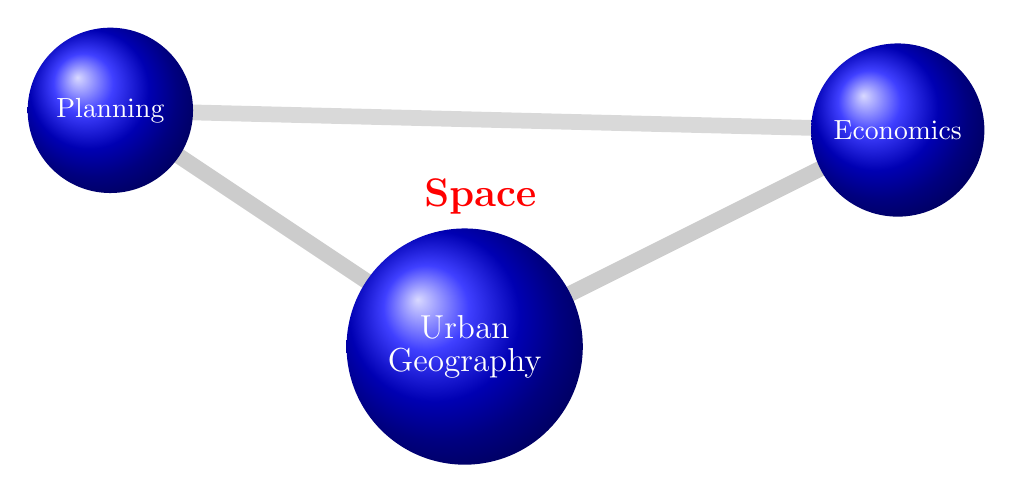
\begin{tikzpicture}{scale=.5}
% find color cotrol for ball. Tind way to stop line short of node
\coordinate (planning) at (-5,1);%PREFACE
\coordinate (economics) at (5,.75);%
 \coordinate (geography) at (-.5,-2); %history
\coordinate (finance) at (0,5); %

\draw [line width=2mm, black!15, ] (planning)--(economics);
\draw [line width=2mm, black!20, ] (geography)--(economics);
\draw [line width=2mm, black!20, ] (geography)--(planning);

%\draw [line width=2mm, black!25, ] (geography)--(finance);
%\draw [line width=2mm, black!20, ] (planning)--(finance);
%\draw [line width=2mm, black!20, ] (finance)--(economics);

\node [circle,shading=ball, minimum width=2.1   cm, white, align=center] (ball) at (planning) {Planning};
\node [circle,shading=ball, minimum width=2.2cm, white, align=center] (ball) at (economics) {Economics};
\node [circle,shading=ball, minimum width=3cm, white, align=center] (ball) at (geography)[text width=2cm] {\large Urban\\ Geography};

%\node [circle, shading=ball, minimum width=2.4cm, white, align=center] (ball) at (finance)[text width=2cm] {Finance};

\node at (-.3,-.1) [red] {\Large \textbf{Space}};
\end{tikzpicture}

Figure 1: The common concern of three fields
topic 

A simple economic insight -- that locational value gives rise to land rents -- provides an organizing principle for the three disciplines where they overlap. Locational value explains the spatial distribution of human activities and the distribution of locational rents goes some distance to explaining  core social issues like class structure, inequality, political political power and the dynamics of economic development.  To understand current changes in our urban system we will examine the development of the relevant theoretical tools, beginning with classical rent theory.


Rent theory has a long history in economics, going back to thinkers such as Richard Cantillon (1680s-1734), François Quesnay (1694–1774), the marquis de Mirabeau (1715–1789) and Anne-Robert-Jacques Turgot (name physiocrat) and Adam Smith (1723-1790) and received its classic statement in Ricardo (1772-1823). Nearly contemporaneous thinker, Johann Heinrich  von Th\"unen (1783-1850) developed a planning model to guide the location of economic activities for an urban-agricultural society.  A version of that model  was reinvented in urban geography by XXX. Alonzo\footnote{We use a version of the well-established model of Alonso (1964), Muth (1969) and Mills (1967), and formalised by Wheaton (1974),}

We link the Alonzo model with more recent work on growth theory starting with Robert Solo's XXX and with the endogenous growth models of Lucas () and draw on Jane Jacobs's insight that endogenous urban growth  is. now driving economic development. Jacobs's insight is empirically supported by recent work in the complexity literature on urban scaling by XXXX ()




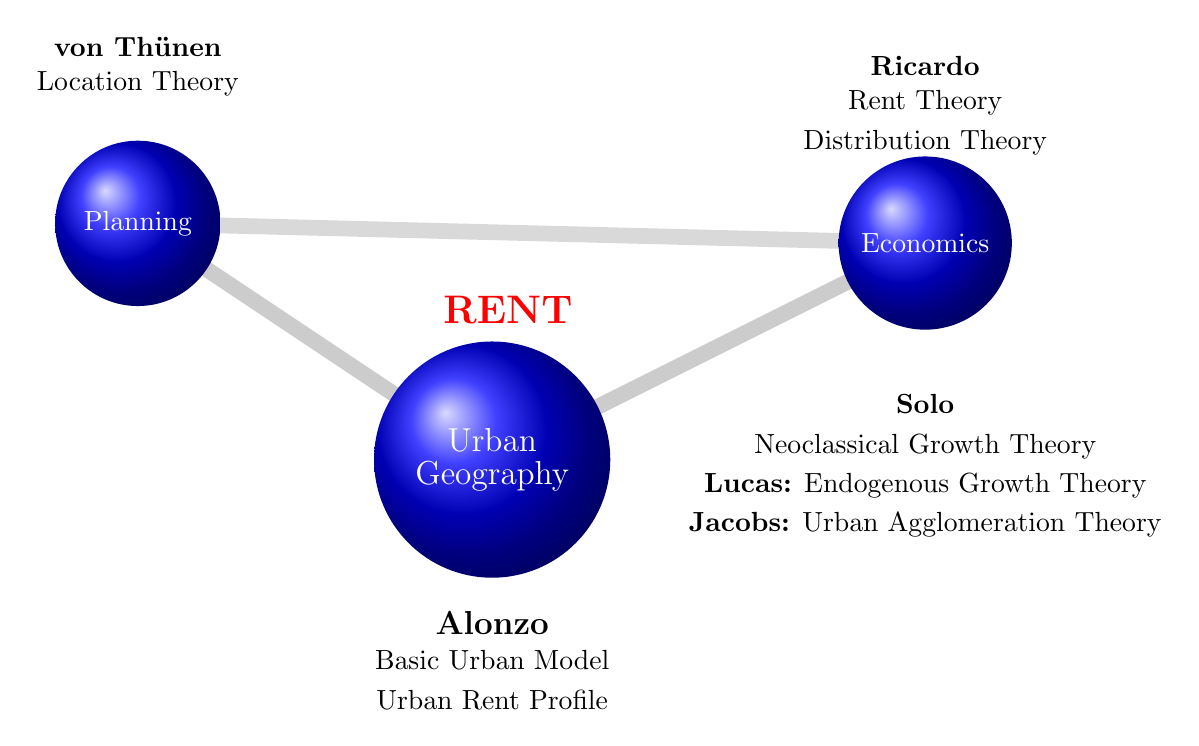
\begin{tikzpicture}{scale=.5}
% find color cotrol for ball. Tind way to stop line short of node
\coordinate (planning) at (-5,1);%PREFACE
\coordinate (economics) at (5,.75);%
 \coordinate (geography) at (-.5,-2); %history
\coordinate (finance) at (0,5); %

\draw [line width=2mm, black!15, ] (planning)--(economics);
\draw [line width=2mm, black!20, ] (geography)--(economics);
\draw [line width=2mm, black!20, ] (geography)--(planning);

%\draw [line width=2mm, black!25, ] (geography)--(finance);
%\draw [line width=2mm, black!20, ] (planning)--(finance);
%\draw [line width=2mm, black!20, ] (finance)--(economics);

\node [circle,shading=ball, minimum width=2.1   cm, white, align=center] (ball) at (planning) {Planning};
\node [circle,shading=ball, minimum width=2.2cm, white, align=center] (ball) at (economics) {Economics};
\node [circle,shading=ball, minimum width=3cm, white, align=center] (ball) at (geography)[text width=2cm] {\large Urban\\ Geography};

%\node [circle, shading=ball, minimum width=2.4cm, white, align=center] (ball) at (finance)[text width=2cm] {Finance};

\node at (-.3,-.1) [red] {\Large \textbf{RENT}};

% new stuff
\node at (planning) [above=2cm] {\textbf{von Th\"unen}};
\node at (planning) [above=1.5cm] {Location Theory};

\node at (economics) [above=2cm] {\textbf{Ricardo}};
\node at (economics) [above=1.5cm] {Rent Theory};
\node at (economics) [above=1.0cm] {Distribution Theory};

\node at (economics) [below=1.8cm] {\textbf{Solo}};
\node at (economics) [below=2.3cm] {Neoclassical Growth Theory};
\node at (economics) [below=2.8cm] {\textbf{Lucas:} Endogenous Growth Theory};
\node at (economics) [below=3.3cm] {\textbf{Jacobs:} Urban Agglomeration Theory};


\node at (geography) [below=1.8cm] {\textbf{\large Alonzo}};
\node at (geography) [below=2.3cm] {Basic Urban Model};
\node at (geography) [below=2.8cm] {Urban Rent Profile};
\end{tikzpicture}

Figure 3: space and value

Land rent was historically the basis of the wealth and political power of  the land-owning class in the era of the classical economists.


We further link the model of urban rents to emerging concerns about the financialization of the housing market. The key insight we offer is that the financialization  of the housing sector is a  form of rent-seeking that must have detrimental effects on urban development and on the well-being of urban residents.





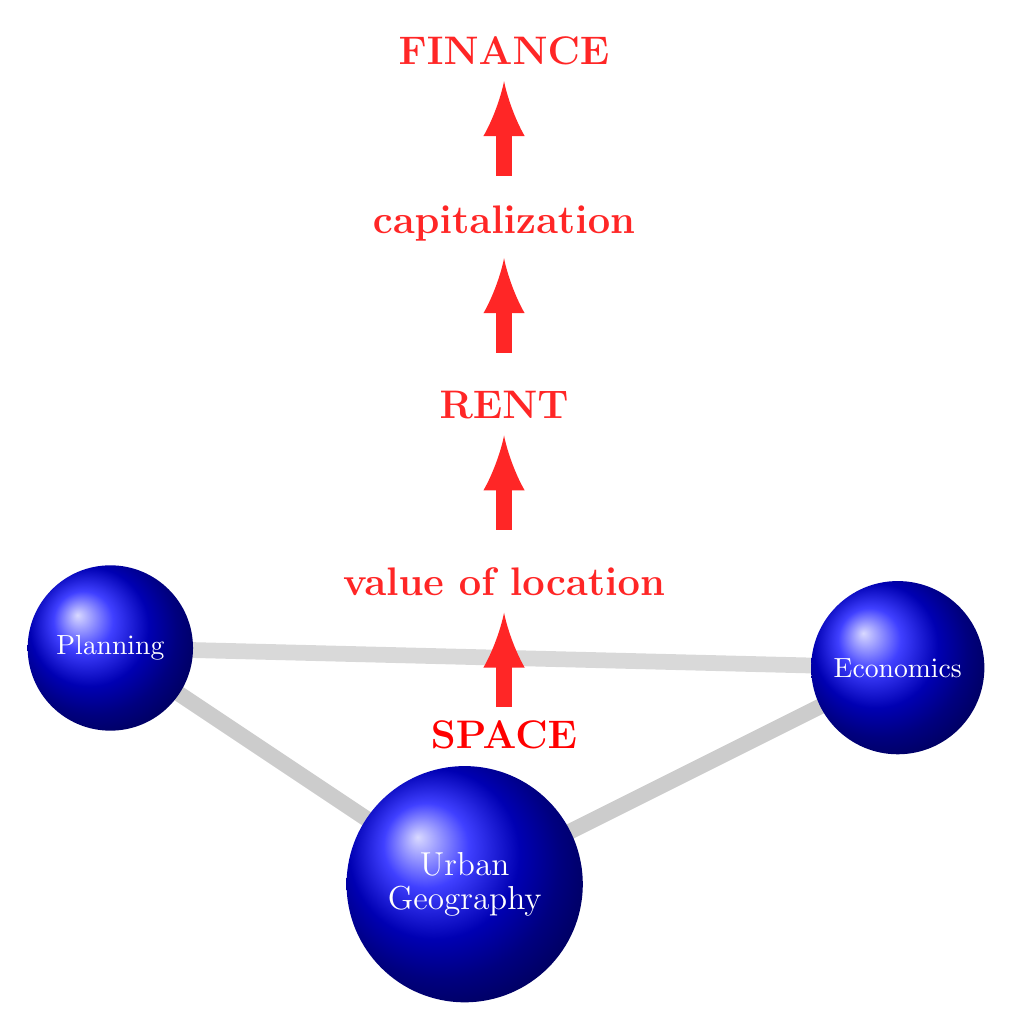
\begin{tikzpicture}{scale=.5}
% find color cotrol for ball. Tind way to stop line short of node
\coordinate (planning) at (-5,1);%PREFACE
\coordinate (economics) at (5,.75);%
 \coordinate (geography) at (-.5,-2); %history
\coordinate (finance) at (0,5); %

\draw [line width=2mm, black!15, ] (planning)--(economics);
\draw [line width=2mm, black!20, ] (geography)--(economics);
\draw [line width=2mm, black!20, ] (geography)--(planning);

%\draw [line width=2mm, black!25, ] (geography)--(finance);
%\draw [line width=2mm, black!20, ] (planning)--(finance);
%\draw [line width=2mm, black!20, ] (finance)--(economics);

\node [circle,shading=ball, minimum width=2.1   cm, white, align=center] (ball) at (planning) {Planning};
\node [circle,shading=ball, minimum width=2.2cm, white, align=center] (ball) at (economics) {Economics};
\node [circle,shading=ball, minimum width=3cm, white, align=center] (ball) at (geography)[text width=2cm] {\large Urban\\ Geography};

%\node [circle, shading=ball, minimum width=2.4cm, white, align=center] (ball) at (finance)[text width=2cm] {Finance};
\draw [line width=2mm, red!85, -latex ] (0, 7)--++(0,1.2)node[above=-.1] {\Large \textbf{FINANCE}};
\draw [line width=2mm, red!85, -latex ] (0, 4.75)--++(0,1.2)node[above=-.1] {\Large \textbf{capitalization}};
\draw [line width=2mm, red!85, -latex ] (0, 2.5)--++(0,1.2)node[above=-.1] {\Large \textbf{RENT}};
\draw [line width=2mm, red!85, -latex ] (0, .25)--++(0,1.2)node[above=-.1] {\Large \textbf{value of location}};
\node at (0,-.1) [red] {\Large \textbf{SPACE}};
\end{tikzpicture}



% \vspace {2cm}
% Figure 4 with finance

% \begin{tikzpicture}{scale=.5}
% % find color cotrol for ball. Tind way to stop line short of node
% \coordinate (planning) at (-5,1);%PREFACE
% \coordinate (economics) at (5,.75);%
%  \coordinate (geography) at (-.5,-2); %history
% \coordinate (finance) at (0,5); %

% \draw [line width=2mm, black!15, ] (planning)--(economics);
% \draw [line width=2mm, black!20, ] (geography)--(economics);
% \draw [line width=2mm, black!20, ] (geography)--(planning);

% \node at (-.3,2) [red] {\huge \textbf{RENT}};

% \draw [line width=3mm,  black!50,opacity=.5 ] (geography)--(finance);
% \draw [line width=2mm, black!20, ] (planning)--(finance);
% \draw [line width=2mm, black!20, ] (finance)--(economics);

% \node [circle,shading=ball, minimum width=2.1   cm, white, align=center] (ball) at (planning) {Planning};
% \node [circle,shading=ball, minimum width=2.2cm, white, align=center] (ball) at (economics) {Economics};
% \node [circle,shading=ball, minimum width=3 . cm, white, align=center] (ball) at (geography)[text width=2cm] {\large Urban\\ Geography};

% \node [circle, shading=ball, minimum width=2.4cm, white, align=center] (ball) at (finance)[text width=2cm] {Finance};


% \end{tikzpicture}



\vspace {2cm}
Figure 4 with finance

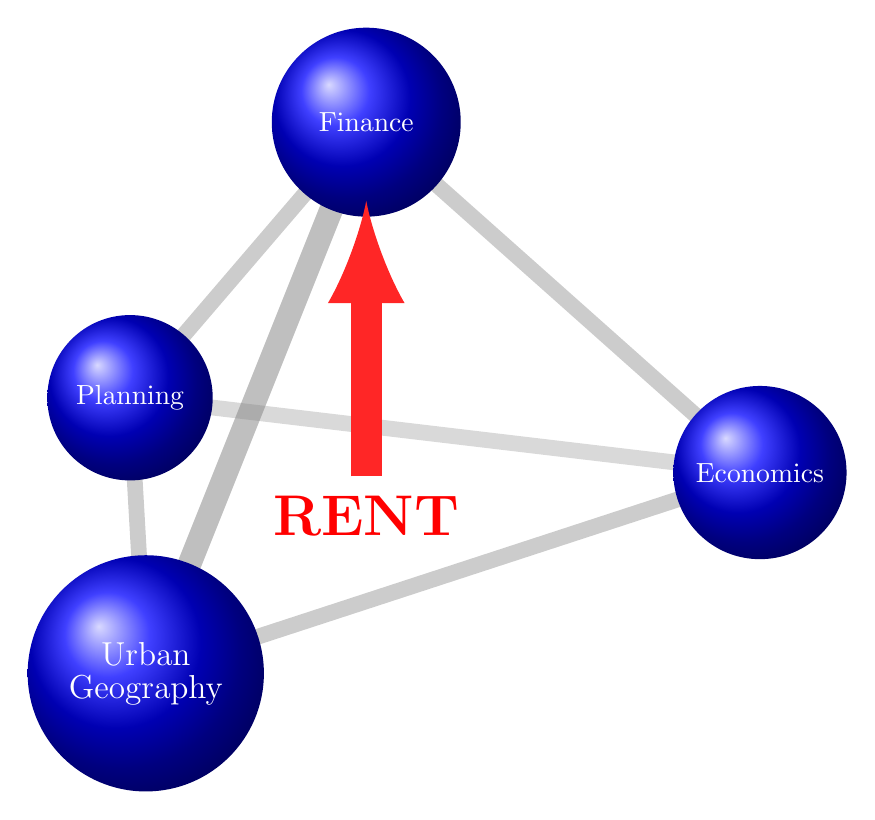
\begin{tikzpicture}{scale=.5}
% find color cotrol for ball. Tind way to stop line short of node
\coordinate (planning) at (-3,1.5);%PREFACE
\coordinate (economics) at (5,.55);%
 \coordinate (geography) at (-2.8,-2); %history
\coordinate (finance) at (0,5); %

\draw [line width=2mm, black!15, ] (planning)--(economics);
\draw [line width=2mm, black!20, ] (geography)--(economics);
\draw [line width=2mm, black!20, ] (geography)--(planning);

\node at (.0,0) [red] {\huge \textbf{RENT}};

\draw [line width=3mm,  black!50,opacity=.5 ] (geography)--(finance);
\draw [line width=2mm, black!20, ] (planning)--(finance);
\draw [line width=2mm, black!20, ] (finance)--(economics);

\node [circle,shading=ball, minimum width=2.1   cm, white, align=center] (ball) at (planning) {Planning};
\node [circle,shading=ball, minimum width=2.2cm, white, align=center] (ball) at (economics) {Economics};
\node [circle,shading=ball, minimum width=3cm, white, align=center] (ball) at (geography)[text width=2cm] {\large Urban\\ Geography};

\node [circle, shading=ball, minimum width=2.4cm, white, align=center] (ball) at (finance)[text width=2cm] {Finance};
\draw [line width=4mm, red!85, -latex ] (0, .5)--(0,4);


\end{tikzpicture}
